\documentclass {aldast}

\usepackage{subfig}
\usepackage{makecell}

\documentType{Lecture Notes}
\documentNumber{1.2}
\title{Random Access Machines}
\author{F. Chauvel}


\begin{document}

\maketitle

\begin{abstract}
  We look at \emph{random access machines} (RAM), a type of machines
  that can carry out computations and that closely resemble an actual
  ``computer'' with a processor and a memory. This model of
  computation will define the elementary capabilities we need for a
  ``computing device'' and how a computation takes place. Then, we
  will look at assembly code and imperative languages, two
  \emph{programming languages}, which we can build for RAM.
\end{abstract}


\section*{Introduction}
We have already clarified several important concepts: Computation,
data, algorithm and data structure. In a nutshell, a computation is a
``mechanic'' transformation of input data into output data. An
algorithm is the sequence of steps that specifies what computation to carry
out in order to solve a computational problem.

What about the \emph{computer}? We saw that anything that can run a
computation fits, but a primary school pupil and an Intel chip does
not really look the same, do they?  In this lecture, we will look at
these ``computing devices''. We will define a model of an ``ideal''
computer, which will help us answering:
\begin{enumerate}
\item What capabilities does our computer has?
\item What does it mean for the computer to use any of these
  capabilities?
\item How can we describe an algorithm for that computer to execute?
\end{enumerate}

This ``ideal'' computer is the \emph{model of computation} which we
will assume in this course. It is called \emph{random access machines}
and underpins all imperative programming languages such as C, Pascal,
Ada, Java, Python, etc. This may is a little theoretical, but this
model of computation will be quite handy when discuss the correctness
and efficiency of algorithms. Other programming paradigms such as
functional programming (e.g., LISP, Haskell, OCaml), logic programming
(e.g., Prolog), hardware circuits or parallel computing use
different models of computation.

I broke down this lecture into two parts. First we look at random
access machines, how they are structured, what they can do, and how we
can instruct them using \emph{machine code}. Then we will see how one
can convert the pseudo code we used in the first lecture into their
machine code.

\section{Random Access Machines}
In this course, the machine we will use is called a \emph{random
  access machine} (RAM)~\cite{cook1973}. It closely resemble an actual
``computer'', with a CPU and a memory, which makes it the\emph{de
  facto} standard in algorithms and data structure course. RAM answers
three questions:
\begin{enumerate}
\item How does the machine acquires, stores and retrieves data?
\item What elementary computation can the machine do?
\item How does the machine follow instructions?
\end{enumerate}

RAM is an abstract machine, a ``model'' of computation: It is a
blueprint for machine that carries out computation. A real computer is
much more complicated.

\subsection{Architecture}

A random access machine (RAM) is a machine that mimics the behavior of
a real computer. It manipulates data encoded as symbols\sidenote{The
  actual alphabet does not matter, as long as we have means to
  implement simple symbol manipulations in hardware}. It has the three
following components, also shown on Figure~\ref{fig:ram}.
\begin{itemize}
\item An \emph{I/O device} that the machine uses to exchange sequence
  of symbols with the user. We can think of this as a screen and a
  keyboard for example.
\item A \emph{memory}, which contains infinitely many
  \emph{cells}. Each memory cell can contains an arbitrary long
  sequence of symbols (i.e., a number) and has a unique identifier (so
  called its address) which will allow to read and write anywhere in
  this memory.
\item A central processing unit (CPU) that carries out arithmetic and
  logical operations (addition, subtraction, comparison, etc.). This CPU
  has two \emph{registers}, namely \texttt{ACC} and \texttt{IP} which
  can both hold any arbitrary long sequence of digits.
  \begin{itemize}
  \item \texttt{ACC} is the \emph{accumulator} and holds
    intermediate results.
  \item \texttt{IP} is the \emph{instruction pointer}, and contains the
    address where the next instruction is located.
  \end{itemize}
\end{itemize}

\begin{figure}[htbp]
  \begin{center}
    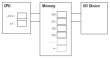
\includegraphics[width=0.8\textwidth]{images/ram}
  \end{center}
  \caption{The architecture of random access machines}
  \label{fig:ram}
\end{figure}

This RAM model remains a gross
simplification\sidenote{TAOCP~\cite{knuth1978} uses a more realistic
  machine model named MIX. If you are curious, ``Code'' by C. Petzold
  \cite{petzold2000} gives a very easy to read account.}. In a
``real'' computer, both the memory cells and the register have a
limited size and can only contain a fixed number of binary digits (8,
16, 32 or 64 bits). This is known as the \emph{word}-size, and
captures the number of symbols the machine processes in one
go. Besides, a real machine also has a limited memory, as well as many
more registers with dedicated purposed.

For the RAM to do anything, we need to tell it what to do. We can
basically instruct it to move symbols from the memory to the CPU, to
apply some elementary symbol manipulations on the CPU's registers and
to move symbol from the CPU back to the memory.

\subsection{Machine Code}
\label{sec:machine-code}

To use our RAM, we need to express our algorithm as a single list of
instructions. Table~\ref{tab:ram-instructions} details the eight
instructions available. Each instruction is a pair of natural numbers,
say $(1, 12)$ for instance. The first one is the \emph{operation code}
(OP) and indicates which action the machine must executed (read,
write, add, etc.). The second number is the \emph{operand} and details
what piece of data the machine must manipulate. So the pair
$(1, 12)$ means \texttt{LOAD 12}, because $1$ is the
operation code of the \texttt{LOAD} instruction, and 12 is the
operand. The machine would thus override the value of the \texttt{ACC}
register with the sequence of symbols ``12'', as explained in
Table~\ref{tab:ram-instructions}

\begin{table}[htbp]
  \begin{center}
    \begin{tabular}{r>{\ttfamily}lp{4cm}>{\ttfamily}p{3.5cm}}
      \toprule
      OP & Mnemonic & Description                                                                                                 & Semantic                          \\
      \midrule
      1  & LOAD n   & Load the value $n$ in the \texttt{ACC} register.                                                            & \makecell[tl]{ACC := n            \\IP := IP + 2 } \\[1cm]
      2  & ADD a    & Add the value contained at address $a$ to the \texttt{ACC} register.                                        & \makecell[tl]{ACC := ACC + Mem[a] \\ IP := IP + 2} \\[1cm]
      3  & SUB a    & Subtract the value contained at address $a$ from the \texttt{ACC} register.                                 & \makecell[tl]{ACC := ACC - Mem[a] \\ IP := IP + 2} \\[1cm]
      4  & STORE a  & Store the value of the \texttt{ACC} register in the memory at address $a$.                                  & \makecell[tl]{Mem[a] := ACC       \\ IP := IP + 2} \\[1cm]
      5  & JUMP a   & Reassign the \texttt{IP} register with the address $a$ only if the \texttt{ACC} register value is positive. & \makecell[tl]{if ACC >= 0         \\ ~~~IP := a \\ else \\ ~~~IP := IP + 2} \\[1.5cm]
      6  & READ a   & Read a value from the I/O device and store it at the given address $a$.                                     & \makecell[tl]{Mem[a] := I/O       \\ IP := IP + 2} \\[1cm]
      7  & PRINT a  & Print the value contained at the given address $a$ to the I/O device.                                       & \makecell[tl]{I/O := Mem[a]       \\ IP := IP + 2} \\[1cm]
      ?  & HALT -   & Stop the machine.                                                                                           & N/A                               \\
      \bottomrule
    \end{tabular}
  \end{center}
  \caption{The eight RAM instructions. \texttt{Mem[a]} denotes the
    value stored in memory at the address $a$. Note that \texttt{LOAD}
    takes a value whereas all other instructions accept an
    address. Any OP outside the range $[1, 7]$ stops the machine.}
  \label{tab:ram-instructions}
\end{table}


\paragraph{Where are these instructions?} These RAM instructions are
stored in the main memory, just like any other data\sidenote{This is
  the core principle behind the Von Neumann architecture: Code is just
  yet another type of data!}. Since each instruction is a pair of
number, a program is just a long list of numbers. Each instruction
thus occupies two contiguous memory cells, one holding the operation
code and one holding the operand. This number are the \emph{machine
  code}.

\begin{takeaway}
  The RAM model defines the actions (i.e., the 8 instructions of
  Table~\ref{tab:ram-instructions}) that the machine understand. In
  this course we will assume an \emph{augmented RAM}, which also
  includes instructions for multiplication, division, exponentiation,
  etc.
\end{takeaway}

\subsection{Execution}
Let us see how does the machine computes. It reads two memory cells
from the address contained in the \texttt{IP} register. Then it
executes this instruction following the semantic given in
Table~\ref{tab:ram-instructions}, and start over. The machine stops
as soon as it meets an unknown operation code.

Table~\ref{tab:ram-example} shows the complete memory layout of a tiny
program that reads two numbers and print their sum. The program stores
the numbers given by the user at addresses 50 and 51 respectively. It
also stores the sum at address 52.

\begin{table}[htbp]
  \begin{center}
    \begin{tabular}{>{\ttfamily}l>{\ttfamily}l>{\ttfamily}l}
      \toprule
      Addresses & Content & Interpretation \\
      \midrule
      00, 01 & 6, 50 & READ 50 \\
      02, 03 & 6, 51 & READ 51 \\
      04, 05 & 1,  0 & LOAD  0 \\
      06, 07 & 2, 50 & ADD  50 \\
      08, 09 & 2, 51 & ADD  51 \\
      10, 11 & 4, 52 & STORE 52 \\
      12, 13 & 7, 52 & PRINT 52 \\
      14, 15 & 0, 0 & HALT \\
      \bottomrule
    \end{tabular}
  \end{center}
  \caption{A sample program laid out in memory. The program reads two
    numbers through the I/O device and prints their sum back to the I/O
    device.}
  \label{tab:ram-example}
\end{table}

Given the memory shown by Table~\ref{tab:ram-example}, provided that
\texttt{IP} is initially set to 0, the RAM proceeds as follows:
\begin{enumerate}
\item The machine reads the memory cells at address 0 and 1 and
  interprets these as \texttt{READ 50}. It thus reads a value through
  the I/O device and stores it at the given address (i.e., 50). It
  then increments \texttt{IP} by 2, which now contains the value 2.
\item With \texttt{IP} holding 2, the machine reads addresses 2 and
  3, which it interprets as \texttt{READ 51}. It thus reads another
  value through the I/O device, stores it at address 51, and then
  increments \texttt{IP} by 2 again.
\item With \texttt{IP} being now 4, the machine reads addresses 4 and
  5, which it interprets as \texttt{LOAD 0}. It thus sets the
  \texttt{ACC} register to 0, and then increments \texttt{IP} by 2.
\item \texttt{IP} now equals 6, The machine reads addresses 6 and
  7, which it interprets as \texttt{ADD 50}. It thus adds the value at
  address 50 to the \texttt{ACC} and then increments \texttt{IP} by 2.
\item \texttt{IP} now contains 8. The machine reads addresses 8 and 9,
  which it interprets as \texttt{ADD 51}. It thus adds the value
  stored at address 51 to the \texttt{ACC} register and then increase
  IP by 2.
\item \texttt{IP} is now 10 and the machine reads addresses 10 and 11,
  which it interprets as \texttt{STORE 52}. It writes the value
  contained in the \texttt{ACC} register into the memory at address
  52. It then increments \texttt{IP} by 2, which now holds 12.
\item It now reads addresses 12 and 13, and interprets it as
  \texttt{PRINT 52}. The machine thus sends the value stored at
  address 52 to the I/O devices. It then increments \texttt{IP} by 2.
\item The next instruction, starting at address 14 stops the machine.
\end{enumerate}

\paragraph{Is this RAM powerful enough?} RAM is a \emph{model of
  computation}: It defines how we carry out computations. We saw
however that different computational problems requires different
algorithms, which in turn, may require different machines. Other
models of computation exist such as Turing machines, finite state
machines, $\lambda$-calculus, cellular automata, etc. If you wonder
whether there is a universal machine that can solve all computational
problems, well, yes. Turing machines is the most powerful computation
model we know so far, and RAM and a few others are as powerful. This
equivalence is known as the Church-Turing thesis. This is a
theoretical question that goes beyond the scope of this course but we
will briefly come back to that (see Lecture 12.2). See any textbook on
Computability Theory \cite{fernandez2009} if you are curious.


\section{Programming Languages}

Now we have a \emph{programmable machine}: We can give instructions as
pairs of numbers and the RAM executes them. Its instruction set is powerful
enough to compute anything computable. The problem is that writing
such long list of numbers (i.e., machine code) is painful and error
prone, to say the least.

\subsection{Assembly Code}

Machine code does not fit humans' capabilities. We do not want to uses
addresses but rather names or labels that are meaningful to the
problem at hand. To cope with this, we can use an \emph{assembly
  language} that is better suited to us and that we can convert to
machine code. An assembly program closely resembles the underlying
machine code but provides the following:
\begin{itemize}
\item \emph{Symbolic names} for memory addresses, so that we can refer
  to them with something that is meaningful to us.
\item \emph{Instruction mnemonics} so that we can refer to machine
  instructions by name rather than by operation code.
\item \emph {Memory Layout} that clearly delineates between memory
  cells that store program instructions from those that store program
  data (input, output, intermediate results).  \marginnote{
    \includestandalone[width=.9\marginparwidth]{images/memory-layout.tikz}
    \captionof{figure}{Separating data from instructions with
      dedicated memory segments. Data goes from address 0 to $k-1$ and
      code from $k$ to $k+i-1$.}
    \label{fig:memory-layout}
  }[-1.5cm]
\end{itemize}

\begin{figure}[htbp]
  \begin{center}
    \begin{minted}{asm}
             .data
             n1    WORD  0   
             n2    WORD  0
             sum   WORD  0
      
             .code
      main:  READ  n1       ; read two numbers n1 and n2
             READ  n2
             LOAD  0        ; add n1 to n2
             ADD   n1
             ADD   n2      
             STORE sum      ; save as "sum"
             PRINT sum      ; show the result
             HALT
    \end{minted}
  \end{center}
  \caption{Assembly code for reading two numbers and printing out
    their sum (see Table~\ref{tab:ram-example})}
  \label{fig:asm}
\end{figure}

Figure~\ref{fig:asm} shows an ``hypothetical'' assembly
program\sidenote{There are roughly as many assembly languages as
  there are processors manufacturers. See \cite{streib2020} for a
  gentle and yet practical introduction.} for our program that reads
two numbers and prints their sum (see Table~\ref{tab:ram-example}). It
defines a data and a code segments (denoted by \texttt{.data} and
\texttt{.code} respectively) as shown on
Figure~\ref{fig:memory-layout}. The data segment defines three
variables \texttt{n1}, \texttt{n2}, and \texttt{sum}, whose size is
one word and whose initial value is ``0''. The code segment contains
eight instructions, using mnemonics instead of operation codes and
symbolic names instead of addresses. The entry point of the code
segment is given the name ``main''. We can use this label ``main'' to
refer to the address of the first instruction.

Now we can use an \emph{assembler}\sidenote{Assembly programs are just
  data (sequence of symbols), so an assembler is another program that
  converts an assembly program into a machine program.} to convert our
assembly code into machine code and get a long list of numbers 6, 50,
6, 51, \ldots, 0, 0 (see Table~\ref{tab:ram-example}) we can feed to
the machine. The actual numbers generated depends on the where the
assembler decides to place the code and data segments into memory.


\subsection{High-level code}

Still writing assembly code is not practical. What we would like is
some sort of pseudocode with control structures such as loops and
conditional statement. These are what we find in general purpose
programming languages such as C, Java or Python. Here are the most
common constructs:
\begin{itemize}
\item \emph{Arithmetic and logic expressions} such as $a + c \geq
  25$. They may refer to variable by name and contains explicit numbers
  (literals).
\item \emph{Assignments} such as $v \gets e$ which assigns the value
  of resulting from expression $e$ the name $v$.
\item \emph{Conditionals} such
  ``$\mathbf{if} \; e \; \mathbf{then} \; c_1 \; \mathbf{else} \; c_2$ which
  executes code $c_1$ only if the expression $e$ holds, and code $c_2$
  otherwise.
\item \emph{Loops} such as ``$\mathbf{while} \; e \; \mathbf{do} \; c$'' which
  executes code $c$ as long as the expression $e$ holds.
\item \emph{Sequence of instructions} such as $c_1 ; c_2$ which
  executes $c_1$ and then $c_2$.
\end{itemize}

We need to translate these constructs into assembly code either
explicitly by a \emph{compiler} or executed line by line by an
\emph{interpreter}. Without diving into the nitty-gritty details of
compilers it is critical to understands this translation scheme.

\begin{takeaway}
  There are \emph{many ways} to encode a given piece of pseudo-code
  into machine code. It is important to understand---at a
  high-level---how a compiler does that.
\end{takeaway}

% \begin{eqnarray*}
%   c \in Command & ::= & \mathbf{while} \; e \; \mathbf{do} \; c_1 \\
%                 & | & \mathbf{if} \; e \; \mathbf{then} \; c_1 \; \mathbf{else} \; c_2 \\
%                 & | & \mathbf{read} \, v \; | \; \mathbf{print} \, e \; | \; \mathbf{skip} \\
%                 & | & v \gets e \\
%                 & | & c_1 \; \mathbf{;} \; c_2 \\
%   e \in Expression & ::= & e_1 + e_2 \; | \; e_1 - e_2 \; | \; e_1 \times e_2 \; | \; e_1 / e_2 \; | \;- e_1\\
%                 & | & e_1 = e_2 \; | \; e_1 < e_ 2 \\
%                 & | & e_1 \land e_2 \; | \; e_1 \lor e_2 \; | \; \neg \, e_1 \\
%                 & | & ( \, e_1 \, ) \; | \;  v \; | \; n \\
%   v \in Variable & ::= & \\
%   n \in \mathbb{N} & & \\
% \end{eqnarray*}

\paragraph{Assignments}
\marginnote{
  \includestandalone[width=.6\marginparwidth]{images/compile-assignment.tikz}
  \captionof{figure}{ASM generated for an assignment $v \gets e$}
  \label{fig:compile-assignment}
} An assignment associates a name to an expression. For example the
assignment ``$\mathit{age} \gets 42$'' associates the label ``age'' to
the number 42. In the general case, the left hand side of an
assignment is an expression: A symbolic name, a number, or an
arithmetic expression (see below). Figure~\ref{fig:compile-assignment}
illustrates one possible assembly code for assignments.
  
\paragraph{Expressions} Evaluating an expression consists in building
a sequence of instructions that leaves the result in \texttt{ACC}
register. The first thing RAM compiler would do is to break long
arithmetic expressions into a sequence of binary assignments, according to the
precedence rules of arithmetic operators. Consider the following
example:

\begin{equation}
  x + (2y + 3) \equiv \left\{
    \begin{array}{rl}
      v_1 & \gets 2 \times y \; ; \\
      v_2 & \gets v_1 + 3 \; ; \\
      \mathit{ACC} & \gets x + v_2 \; ;
    \end{array} \right.
\end{equation}

\begin{itemize}
\item If the given expression is a single number $n$, then a
 single \texttt{LOAD} instruction suffices, and the compiler just emits
  $\mathtt{LOAD} \; n$. It directly sets \texttt{ACC} with $n$ as
  shown on Figure~\ref{fig:compile-literal}.
\item If the given expression is a symbolic name, say $v$ for
  instance, then, we need two instructions: One to reset the
  \texttt{ACC} register to zero and another one to add the value
  contained at the address associated with the given
  symbol. Figure~\ref{fig:compile-variable} illustrates this case.
\item If the expression is an arithmetic operation, say
  ``$e_1 + e_2$'' for instance, we have to first evaluate $e_1$, and
  store the result in a temporary location, then evaluate $e_2$ and
  store the result in another temporary location and finally, add
  these two temporary values
  together. Figure~\ref{fig:compile-addition} shows the assembly code
  yielded for an addition.
\end{itemize}


\begin{figure}
    \centering
    \subfloat[Single number $n$]{
      \includestandalone[width=.6\marginparwidth]{images/compile-literal.tikz}
      \label{fig:compile-literal}
    }
    \qquad
    \subfloat[Single variable $v$]{
      \includestandalone[width=.6\marginparwidth]{images/compile-variable.tikz}
      \label{fig:compile-variable}
    }
    \qquad
    \subfloat[Expression $e_1 + e_2$]{
      \includestandalone[width=.6\marginparwidth]{images/compile-addition.tikz}
      \label{fig:compile-addition}
    }
    \caption{Evaluation of expressions. After these instructions, the
      \texttt{ACC} register contains the value of the given
      expression.}
    \label{fig:compile-expressions}
\end{figure}


\paragraph{Sequences of commands}
\marginnote{
  \includestandalone[width=.6\marginparwidth]{images/compile-sequence.tikz}
  \captionof{figure}{ASM generated for a sequence of commands $c_1 \, ; \, c_2$}
  \label{fig:compile-sequence}
} A sequence of code blocks ``$c_1 \, ;\, c_2$'' specifies the
execution order of these two blocks. To this end, we either place the
ASM code for $c_2$ right after the one for $c_1$ (as shown on
Figure~\ref{fig:compile-sequence}), or place a \texttt{JUMP} in
between.


\paragraph{Conditionals} A conditional selects between two blocks of
code $c_1$ and $c_2$ depending on the evaluation of an expression
$e$. To compile these, we need first to compile this expression
$e$. In case this expression does not hold, we ``jump''
to the code resulting from the compilation of the ``else'' block
$c_2$. Otherwise we continue with the ``then'' $c_1$ block
followed by a \texttt{JUMP} to the end of the
conditional. Figure~\ref{fig:compile-conditional} illustrates this
layout.

\paragraph{Loops} Finally, a loop executes a given block of code $c$
as long as the guard expression $e$ holds. To do that, we place the
code to evaluate the expression $\neg \, e$, followed by a
\texttt{JUMP} to the end of the loop, in case the expression does not
hold. Then, we append the assembly code of $c$ followed by a
\texttt{JUMP} back to the evaluation of the guard expression, as shown
in Figure~\ref{fig:compile-loop}.


\begin{figure}
    \centering
    \subfloat[$\mathbf{if}\; e \; \mathbf{then} \; c_1 \; \mathbf{else} \; c_2$]{
      \includestandalone[width=.8\marginparwidth]{images/compile-conditional.tikz}
      \label{fig:compile-conditional}
    }
    \hfill
    \subfloat[$\mathbf{while}\; e \; \mathbf{do} \; c$]{
      \includestandalone[width=.8\marginparwidth]{images/compile-loop.tikz}
      \label{fig:compile-loop}
    }
    \caption{Compilation of loops and conditionals using \texttt{JUMP} and labels.}
    \label{fig:compile-control}
\end{figure}

\begin{takeaway}
  A \emph{program} is an algorithm encoded using \emph{a programming
    language}. This program can be converted into \emph{machine code}
  for execution by a computing device.
\end{takeaway}

\subsection{Example}
\label{sec:example}

Now we can describe an algorithm in pseudo code and understand what
assembly code and machine could possibly execute this
program. Returning to the multiplication of two natural numbers,
Figures~\ref{alg:product} and~\ref{asm:product} show the pseudo code
and some possible assembly code. During the compilation, we assume
that input are read from the I/O device and output printed.

\begin{figure}
  \marginnote{%
    \scalebox{0.9}{
      \begin{minipage}{1.1\marginparwidth}
      \begin{algorithm}[H]
        \KwIn{$(x, y) \, \in \, \mathbb{N}^2$}
        \KwOut{$y = x \times y$}
        $product \gets 0$\;
        $counter \gets 0$\;
        \While{$\mathit{counter} < y$}{
          $product \gets product + x$\;
          $counter \gets counter + 1$\;
        }
        \Return{$product$}
      \end{algorithm}
      \end{minipage}
    }
    \captionof{figure}{Pseudo-code of an algorithm that computes the
      product of two natural numbers}
    \label{alg:product}
  }
  \centering
  \inputminted{asm}{code/multiplication.asm}
  \caption{Possible RAM assembly code to multiply two numbers $x$ and $y$, derive from the algorithm given on Figure~\ref{alg:product}}
  \label{asm:product}
\end{figure}


\section*{Conclusion}
We now know the difference (and the relationships) between a problem,
an algorithm and a program. We also know how a machine can store and
execute algorithms using programs written in machine code. Next, we
will see how one can establish the correctness of an algorithm:
Providing evidences that an algorithm actually solves a given problem.


\bibliographystyle{acm}
\bibliography{references}

\end{document}